\begin{frame}{Project objectives}

    Magnetic Levitation System (MLS) it's an electromechanical system that enhances magnetic fields to levitate a ferromagnetic object.
    It's known for its non-linear behavior and its instability.

    \begin{columns}[c, onlytextwidth]

        \begin{column}{0.5\textwidth}

            \begin{figure}[H]
                \centering
                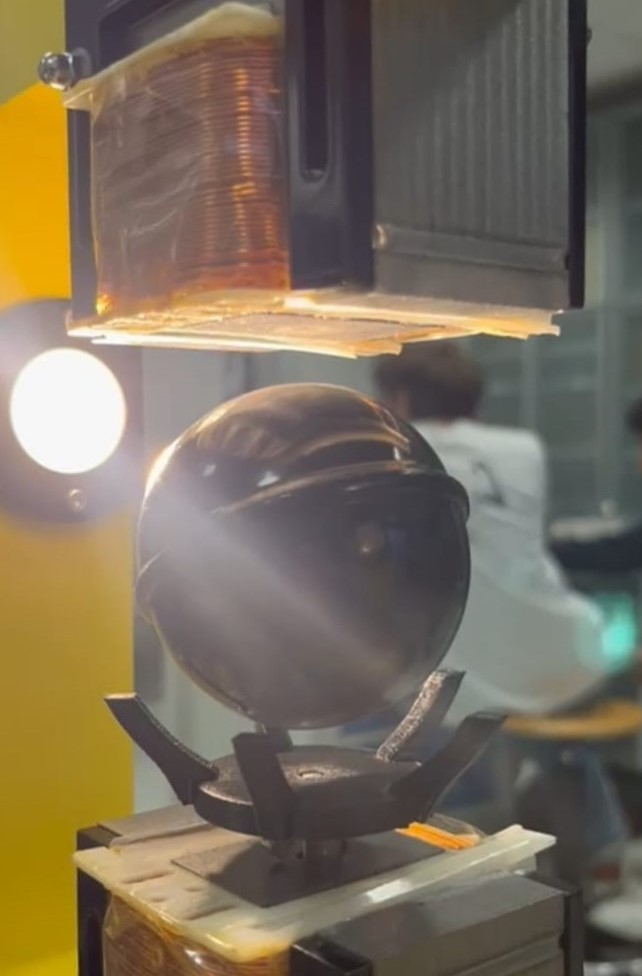
\includegraphics[width=0.7\textwidth]{img/ball_levitation.jpg}
            \end{figure}

        \end{column}

        \begin{column}{0.5\textwidth}

            \begin{center}
                Project objectives: \\
                \textbf{Make the ball levitate.}
            \end{center}

        \end{column}

    \end{columns}



\end{frame}